\chapter{Theoretische Grundlagen}

\section{Energy Harvesting mit Bewegungsinduktion}
HarvesterSchaltung ist durch Machbarkeitsstudie vorgegeben.
Kurze Einführung der von uns optimierten Schaltung. 





\section{Konzept des Energy Management der gewonnenen Energie}
In der Bachelorarbeit ist die Entwicklung des Enerergymanagements mit diesem Board vorgegeben.
Links zu anderen PowerManagementSystemen: Booster TI, Analog Devices, E-Beas.


Energy Management bezeichnet das Regeln von Energiezuständen, damit ein Optimum an Leistung aus einer Quelle bezogen werden kann.

EM Microelectronics aus Marin (NE) entwickelt den Energymanagement-Chip EM8500 für Low Power-Anwendungen. 

The EM8500 is an autonomous power management system able to manage power domains, power sources and storage elements \cite{datasheet_EM85}, p. 11.

Zu diesem Chip ist das Evaluation-Board EMEVB8500 entwickelt, welches das Aufsetzen eines energieoptimierten Systems unterstützt. 


\subsection{Regelung des optimalen Leistungsbezugs}

Wichtigster Punkt in der Energieoptimierung ist das Leistungsverhalten der Quelle. Zu jeder Quelle gehören MaximumPowerPoints (MPP), die Punkte, an denen am effizientesten Leistung bezogen werden kann. 

Das Evalutions-Board von Microelectronics (im Text mit EVB abgekürzt) versucht die Quelle stets in der Nähe dieses Optimums zu betreiben. Dies macht das EVB so, in dem es zu jeder Eingangsspannung intern den Innenwiderstand auf dem EVB so regelt, dass über den geregelten EVB-Strom die Eingangsleistung möglichst dem MPP entspricht.


Neben der Optimalen Leistungsnutzung ist das Ziel der Regelung, konstante Eingangsspannungen zu erzwingen. Das System kontrolliert periodisch den aktuellen (unregulierten) Spannungswert der Harvestingquelle. Hat sich der Wert mehr als 37 mV gegenüber der zur Zeit aktuellen Regelspannung geändert, wird der neue Wert als Spannungsreferenz zum Regeln genommen. Die Abbildung \ref{RegelungSpannung} zeigt das Anpassen der Spannungslevel alle s. Die periodischen Kontrollmessungen alle 8 s verursachen kurze Spannungsspitzen. Diese entstehen bei der Kurzschlussmessung, für den akutellen Stromwert.

\begin{figure}
    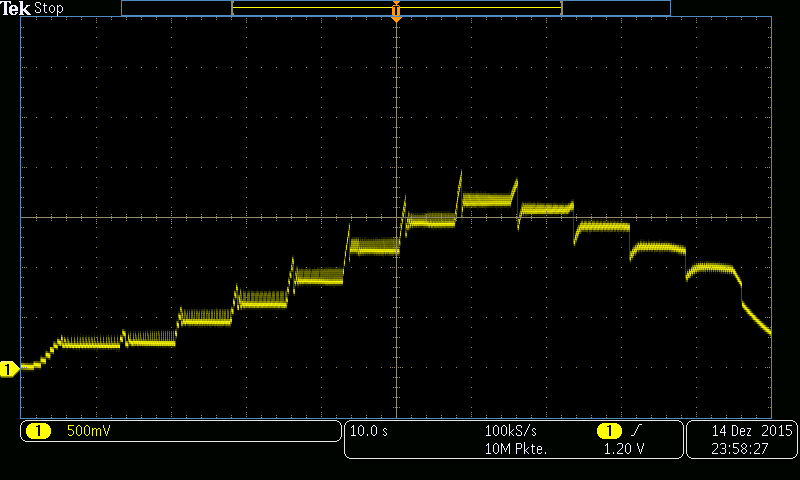
\includegraphics[bb = 0 0 100 100]{2TheoretischeGrundlagen/imag/RegelungVHRV.png}
    \caption{Spannungswerte Modell der Machbarkeitsstudie}\label{RegelungSpannung} 
\end{figure}

Entsprechen die Konfigurationen auf dem EVB nicht dem Verhalten der Eingangsquelle, so entstehen keine konstanten Spannungswerte an der Harvestingquelle, was Abbildung \ref{falscheRegelung} zeigt.

\begin{figure}
    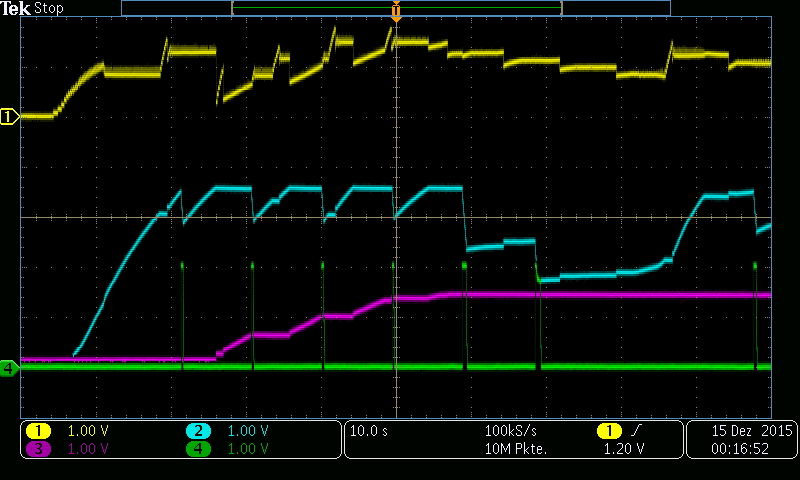
\includegraphics[bb = 0 0 100 100]{2TheoretischeGrundlagen/imag/falscheRegelung.png}
    \caption{Spannungswerte Modell der Machbarkeitsstudie}\label{falscheRegelung} 
\end{figure}

Ausgelassen: Details zur Open Voltage und zur Kurzschluss-Messung.




\subsubsection{Kommunikation mit anderem Bauteil}

Sobald genügend Startenergie bereit steht, wacht der EM8500-Chips auf. Neben dem Setzen der Konfigurationen aus dem EPROM kontrolliert der Chip als erstes den aktuellen Speicherzustand der angeschlossenen Speicher.

Die Engeriequelle wie auch die angeschlossenen Speicher haben eigene Pins, die ihren Zustand übermitteln\cite{datasheet_EM85}, p.11. 




\section{Low Power Microcontroller }
Das TI Sensortag ist vorgegeben. Im Rahmen der Bachelorarbeit nicht möglich, Kontroller zu evaluieren. Dieser hat viele Sensoren.
Grund ist die hohe Rechenleistung. Die mögliche Erweiterung auf Zigbee. 

\section{Bluetooth Low Energy}





